\ifdefined\speakernotes
	\documentclass[notes=only]{beamer}
\else
	\documentclass{beamer}
\fi


\usepackage{hyperref}
\usepackage{listings}
\usepackage{color}
\definecolor{mygreen}{rgb}{0,0.6,0}
\definecolor{mygray}{rgb}{0.5,0.5,0.5}
\definecolor{mypurple}{rgb}{0.8,0,0.8}


% Beamer config
\usefonttheme{serif}
\usetheme{Berkeley}
\usecolortheme{seahorse}

% Set listings defaults
\lstset{    language=[LaTeX]TeX, 
            basicstyle=\scriptsize, 
            keywordstyle=\bfseries\color{blue}, 
            commentstyle=\it \color{red}, 
            numbers=left, 
            alsoletter={\textbackslash},
            numberstyle=\tiny\color{mygray}, 
            numbersep=3pt, 
            literate= {\{}{{{\bf\color{mygreen}\{}}}1 {\}}{{{\bf\color{mygreen}\}}}}1 {\\}{{{\bf\color{blue}\textbackslash}}}1 {\$}{{{\bf\color{magenta}\$}}}1 {\&}{{{\bf\color{orange}\&}}}1 {\~}{{{\bf\color{blue}$\sim$}}}1 {\[}{{{\bf\color{mypurple}[}}}1 {\]}{{{\bf\color{mypurple}]}}}1, 
            breaklines=true, 
            morekeywords={\title, \documentclass, \author, \date, \begin, \end, \textbf, \textit, \emph, \underline, \texttt, \section, \item, \noindent, \sum, \limits, \infity, \omega, \dfrac, \cdot, \pi, \sqrt, &, \hline, \ref, \usepackage, \includegraphics, \centering, \caption, \cite, \bibliography, \bibliographystyle, \bf, \it, \color, \tiny,\footnotesize, \label, \textwidth, \infty, maketitle, subsubsection, subsection, thesection, lstinputlisting, @article, author, title, journal, issue, pages, volume, year}
        }

% define some commands

\newcommand{\snip}[1]
{
	\lstinputlisting[basicstyle=\normalsize, numbers=none]{Resources/Snips/#1}
}

% \codeframe:  creates a frame with code on left and result (image) on right
% args: 1=Title on frame, 2=example name, 3=starting line, 4=ending line, 5=notes
\newcommand{\codeframe}[5]
{
    \begin{frame} \frametitle{#1}
        \begin{columns}[T]
            \column{.52\textwidth}
                \textbf{Source}
                \lstinputlisting[firstline=#3, lastline=#4]{Examples/#2.tex}
            \column{.46\textwidth}
                \textbf{Output}
                \fbox{\includegraphics[width=\textwidth]{Examples/#2.png}}
        \end{columns}
        \note{#5}
    \end{frame}
}

% \pc:  (print command) having to type \textbackslash \{ \} every 
% time I want to include a LaTeX command is horrible.  This makes it less horrible.
\newcommand{\pc}[1]
{
    \texttt{\textbackslash #1}
}

% Presentation Title block
\title{How do \LaTeX?}
\subtitle{\url{https://github.com/ekrause/LaTeX-Presentation}}
\author{Eric Krause}
\institute[PSU]{Portland State University\\\it{M.S. ECE, 2013}}

\begin{document}
\maketitle

\section{Why \LaTeX?}


\begin{frame} \frametitle{Why use \LaTeX?}
    \begin{itemize}
        \item High quality output
        \item Unparalleled math/equation typesetting
        \item Powerful bibliography management 
        \item Handles massive documents with ease
        \item Free and OS agnostic
        \item You get to use your favorite text editor
        \item Highly extensible
        \item \textbf{Focus on content, not formatting}
    \end{itemize}
    
    \note{  -- Latex looks amazing.  \\
    		-- MathType doesn't look as horrendous as it used to, but nothing beats latex for refinement/polish.  It is the mathematical typesetting standard in all technical disciplines and in many related fields. publications in math, computer  science, engineering, and physics\\
            -- bibliography software is usually an extra expense (e.g. EndNote).  BibTex is fast, integrated, and powerful.\\
            -- once you start working on 20+ page documents with tons of pictures and tables (and partners, but that's another story) Word is simply not a viable option.  And by non-viable, I don't mean hard to use? I mean it will crash.  And if it doesn't, you'll wish it did.\\
            -- Free, works on everything, in most if not all linux repos.\\
            -- plain text: vim, sublime text, notepad++, or even Emacs\\
            -- Tons of packages to do everything: code listing, create graphics, write music, whatever \\
            -- Most important:  Allows you to focus on content, not formatting.  \\
    }
\end{frame}


\begin{frame} \frametitle{Don't use LaTeX if...}
    \begin{itemize}
        \item Never used a computer before
        \item Can't spare a few hours of practice in exchange for a life changing skill
        \item Never need to create documents (why are you here?)
        \item Afraid of the command line
        \item Weak, lazy, other personal flaws
    \end{itemize}
    \note{in the beginning it might seem like it's too much work for short documents but with a little practice its really not bad and you'll find yourself using it even for simple things because \textbf{you know it will work every time}.  }
\end{frame}

\section{Getting Started}
\begin{frame} \frametitle{Downloading and Using \LaTeX}
    \textbf{Downloading}
    \begin{itemize}
        \item \textbf{Linux} Check your software repository.
        \begin{itemize} \item \texttt{sudo apt-get install texlive-full} \end{itemize}  
        \item \textbf{OS X} MacTex
        \begin{itemize} \item \url{http://www.tug.org/mactex/}
        \item \texttt{brew install pdflatex} \end{itemize}
        \item \textbf{Windows} ProTexT
        \begin{itemize} \item \url{http://www.tug.org/protext/} \end{itemize}
    \end{itemize}
        
    \textbf{Compiling [command line]}
    \begin{itemize}
        \item {\scriptsize \texttt{pdflatex -file-line-error -interaction=nonstopmode yourfile.tex}}
    \end{itemize}

    \textbf{Compiling [GUI]}
    \begin{itemize}
            \item Click buttons and/or mash keyboard.  
            \item If that doesn't work, try touching the screen or using voice commands.
    \end{itemize}
    \note{-file-line-error = file:line:error style messages. -interaction=nonstopmode = go back to command line on error. When pdflatex can't compile a file, it drops into a prompt. I've never used it and always try to get away from there as quickly as possible, usually generating a q.log file in the process.\\
    - so just use these options for the standard compiler interaction you know and love
}
\end{frame}


\codeframe{Hello \LaTeX!}{1-hello}{1}{16}
{-always have to state the class or type of the thing you are writing (book, article, etc...)\\
- title, author, date store information about your document to use later.  Anything before begin(document) is the preamble\\ 
- the actual document content (anything appearing on the page) happens between begin/end document.\\
-on line 8 the stored info is used in creation of title page\\
\textbf{question}  any guesses on what happens to content after end document?}

\begin{frame} \frametitle{Function Syntax}
    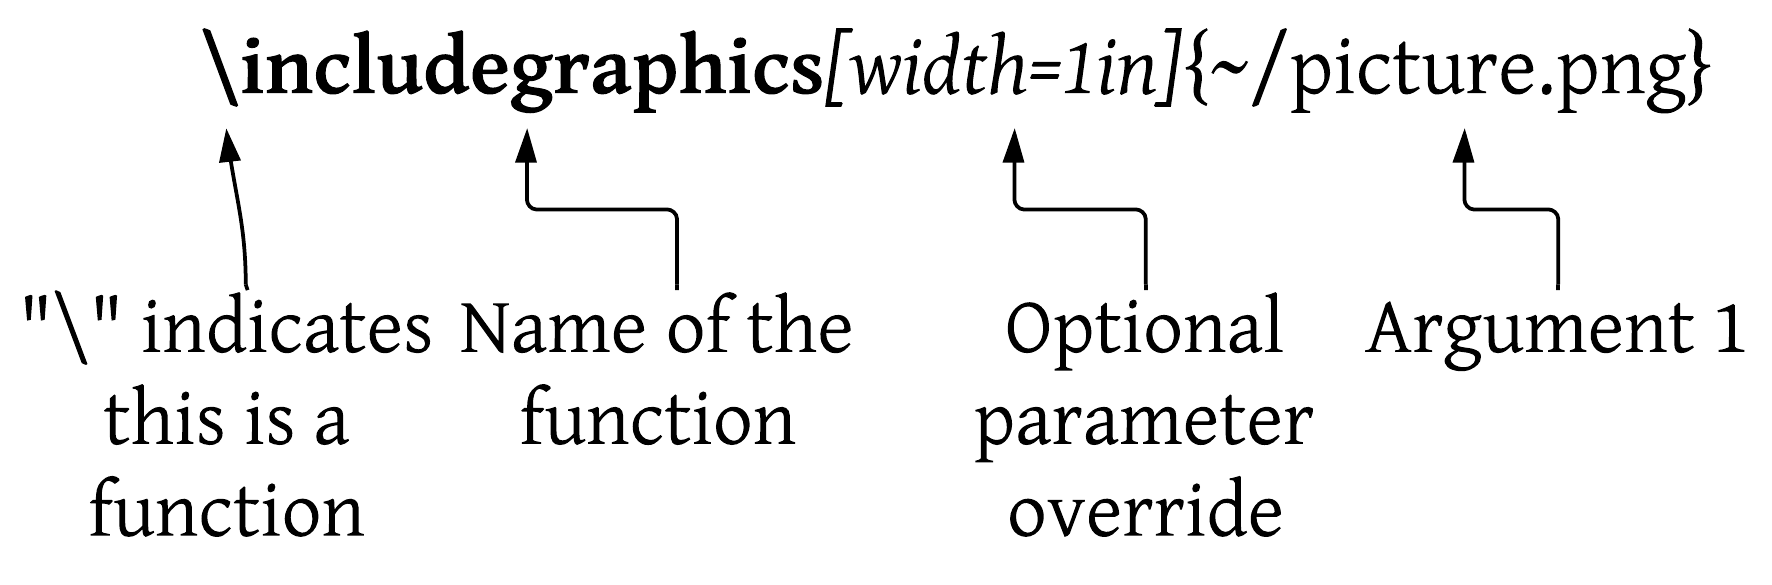
\includegraphics[width=\textwidth]{Examples/0-syntax.png}
    \note{
    -If not giving any optional arguments, don't need to include the empty set of brackets and in my code I do not.\\
    -If more than one optional argument, comma separated list (key-value system)\\
    -If there were more required arguments, each would be in a set of curly braces. \\
    - Required arguments are positional\\
    \textbf{question} how do I pass nothing as an argument? }
\end{frame}

\begin{frame} \frametitle{Spaces and Escaped Characters}
\begin{itemize}
        \item Additional spaces between words are ignored.
        \item Manually add spaces by escaping a space \texttt{`\textbackslash\ '}
        \item Line break: (no indent) two backslashes \texttt{`\textbackslash\textbackslash'}
        \item Paragraph break (indent) two newlines (\texttt{`Enter'} twice)
    \end{itemize}
    
    \small
    \begin{tabular}{| l | l | l |} \hline
                            & \textbf{Unescaped Function}           & \textbf{To Print, Type:}  \\\hline
        \textbackslash      & escape character, command identifier  & \pc{textbackslash}        \\\hline
        \{ \}               & group and separate commands           & \pc{\{} and \pc{\}}       \\\hline
        \%                  & begin a line comment                  & \pc{\%}                   \\\hline
        \$                  & enter/leave math mode                 & \pc{\$}                   \\\hline
        \_                  & for subscripts (math mode)            & \pc{\_}                   \\\hline
        \textasciicircum    & for superscripts (math mode)          & \pc{textasciicircum}      \\\hline
        \&                  & designate columns in tables           & \pc{\&}                   \\\hline
        \#                  & reference arguments in functions      & \pc{\#}                   \\\hline
        \textasciitilde     & insert unbreakable space              & \pc{textasciitilde}       \\\hline
    \end{tabular}
    \note{
    -Spaces are ignored\\
    -Difference between line breaking and paragraph breaking is that paragraph breaks cause an indent.\\
    -Not going to go through this in detail, basically backslash is escape character and also designates the start of a command or function.\\
    -If you try to type one of these and don't escape it you will likely have problems\\
    \textbf{question} what happens if I escape characters other than these?}
\end{frame}


\section{Formatting}

\codeframe{Common Text Formatting}{2-formatting}{4}{10}
{-Text bold font, text italic font, emphasize, underline, text typewriter text\\-Emph takes into account the format where it is used instead of always blindly italisizing}

\codeframe{Sections and Subsections}{3-section}{5}{16}{
-can nest as much as you like.\\
-numbers tracked automatically unless using starred version of command.\\
-note that these are for the article document class.  the book class has chapters and possibly more.\\
-if you ever need deeper nesting, there are additional packages to accomplish this.\\
\textbf{question} what would happen if there were another section after appendix?}

\codeframe{Lists}{4-lists}{4}{19}{
- can nest as much as you like (no limit like sections), but must end environments in the order they are started.  i.e. description enum item ... item enum description\\
- description has an optional argument that basically isn't optional.}

\begin{frame}
    \frametitle{Formatting Miscellanea}
    \begin{itemize}
    \item Quotes:\\
    Backtick (\ \`\ ) for open quote, single quote (\ \'\ ) for close quote.  `single' or ``double''\\
    \item Centering\\
    	\snip{center.tex}
    \item Verbatim\\
     \snip{verbatim.tex}
    \end{itemize} 
    \note{- the double-quote key will still work but the quotes will not open/close.  Also, depending on compilation and other editor settings, you can see weird things like upside-down question marks where your apostrophes should be\\
   	- verbatim is awesome but don't use it for source code, there are better options covered later. } 
\end{frame}


\section{Math Mode}

\begin{frame} \frametitle{Math Mode}
    \begin{itemize}
    	\item \url{http://en.wikibooks.org/wiki/LaTeX/Mathematics}
        \item Begin and end \underline{inline} equations: \vspace{-6pt}
        \begin{itemize} \snip{inline.tex} \end{itemize}\vspace{-10pt}
        \item Begin and end \underline{display} equations:
        \begin{itemize} \snip{displayequation.tex} \end{itemize}
        \item The only symbols accessed directly from the keyboard:  
        \begin{itemize} \item \textit{+ - = ! / ( ) [ ] $< >$ $|$ $'$ :} \end{itemize}
        The rest are all commands!
        \item Spaces are ignored entirely in equations.
        \item How to remember them all?  Don't!  Use \textbf{Dextrify}!
        \begin{itemize} \item \url{http://detexify.kirelabs.org/classify.html} \end{itemize}
    \end{itemize}
    \note{
    -There are lots of symbols in math, very few are accessed using keyboard in LaTeX.  The rest are all commands started with slash.\\
    -Hard to remember all of them, but with Dextrify they are easy to find if you can draw what you are looking for. \\
    \textbf{demo} show how dextrify works.}
\end{frame}

\begin{frame} \frametitle{Math Mode Examples}
    Output:
    \fbox{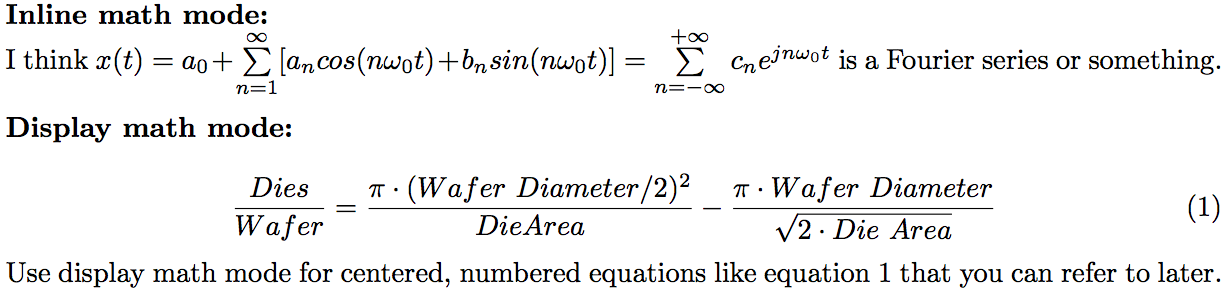
\includegraphics[width=\textwidth]{Examples/5-math.png}}

    Source:
    \lstinputlisting[basicstyle=\tiny, firstline=6, lastline=15]{Examples/5-math.tex}
    
    \note{
    - usepackage(mathtools) required for dfrac (double line fraction)\\
    - probably too small to see, but this serves as a basic example.  Math is one of the strongest features in LaTeX, it can handle anything.\\
    - can't comprehensively cover math mode here but most of it is just knowing the right commands (many of which are intuitive, frac for fraction), and knowing the commands for the symbols you want (dextrify)\\
    \textbf{question} why are there slashes after certain words?}
\end{frame}


\section{Tabular Mode}

\begin{frame} \frametitle{Using the Tabular Environment}
    \begin{enumerate}
        \item \textbf{Begin tabular mode} specifying the number of columns, alignment, and vertical lines.
        \item \textbf{Input table rows} indicating separations between cells, specifying when to begin a new row, and where to include horizontal lines.
        \item \textbf{End tabular mode}
    \end{enumerate}
\end{frame}

\begin{frame} \frametitle{Beginning A Tabular Environment}
    Started using the following command:\\
    \snip{tabular.tex}
    \begin{itemize}
        \item The environment we are starting is \texttt{tabular}.
        \item The type, location, and alignment of columns and vertical lines is given using the \texttt{column specification}
	    \begin{itemize}
	        \item l --- left-aligned column
	        \item c --- center-aligned column
	        \item r --- right-aligned column
	        \item p\{width\} --- paragraph column, must specify width.
	        \item $|$ --- vertical line ($||$ = double, $|||$ = 	triple ...) 
	    \end{itemize}
    \end{itemize}
    \note{
    - width of columns will be automatically fitted to content.\\
    - there is actually an optional placement suggestion between begin(tabular) and the specification, this is covered later in Floats.\\
    - Use paragraph columns to manually control column width.  Text will wrap in paragraph columns.\\\textit{(If text flows out of the table, try using this).}}
\end{frame}

\begin{frame} \frametitle{Adding Contents}
    \begin{itemize}
    	\item Once in a tabular environment, table contents, separations between cells, and newlines are entered.\\
    	\begin{itemize}
			\item \texttt{\&} --- column separator
			\item \texttt{\textbackslash\textbackslash} --- start new row
        	\item \pc{hline} --- horizontal line
			\item \pc{newline} --- start new line in cell (paragraph cells only)
		\end{itemize}
    \end{itemize}
    
    \textbf{Sample Table:}
    \lstinputlisting[firstline=5, lastline=11]{Examples/6-tables.tex}
    \note{
    \textbf{question}\\
    - what will this table look like? \\ 
    - How many columns and rows?\\
    - Justification in each column?\\
    - Where will lines be?}
\end{frame}

\begin{frame} \frametitle{Tabular Example}
    Output:
    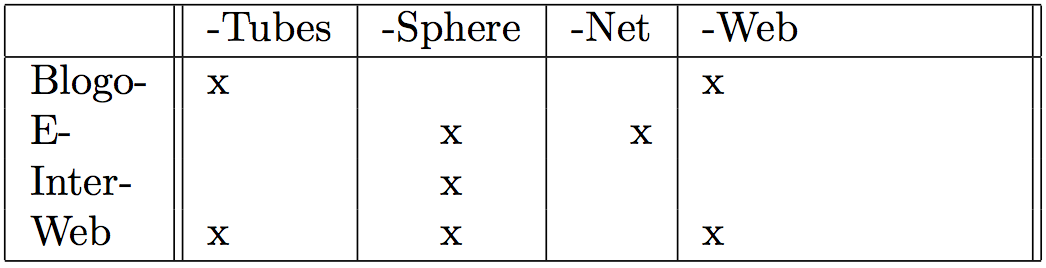
\includegraphics[width=\textwidth]{Examples/6-tables.png}
\end{frame}


\section{Graphics}
    \begin{frame}
    \frametitle{Importing Graphics}
    \begin{itemize}
        \item \snip{graphicx.tex}
        \item Once \texttt{graphicx} is included, images are imported using:\\	
        \snip{includegraphics.tex}
        \item Useful optional parameters:
        \begin{itemize}
            \item width=xx --- manual width
            \item height=xx --- manual height
            \item angle=xx --- used to rotate image
            \item scale=xx --- manual scaling
        \end{itemize}
            
        \item \snip{textwidth.tex}\ \\
        \item \snip{05textwidth.tex}
    \end{itemize}
    \note{
    - LaTeX cannot manage pictures directly, must use the \texttt{graphicx} package. Include graphicsx in preamble of document\\ 
    - textwidth is a really great command to know, it is a macro equal to the width of the printable area.  I considered giving it its own slide but just know that dynamically determining widths and heights is nearly always the correct way to do things.}
\end{frame}

\codeframe{Includegraphics Example}{7-images}{1}{6}
{}


\section{Floats}

\begin{frame} \frametitle{Floats}
    \begin{itemize}
        \item A container that cannot be broken across multiple pages
        \item \LaTeX\ defines \texttt{figure} and \texttt{table} floats
        \item Floats (should) have captions and references.
        \item Floats are automatically arranged by \LaTeX\ , however you can manually specify placement
    \end{itemize}
\end{frame}

\begin{frame} \frametitle{Float Placement}
    \textbf{Format:}\\
    
    
	\snip{snip_float.tex}\vspace{-6pt}

    \begin{itemize}
        \item To get number of the float: \vspace{-6pt}\snip{ref.tex}  
        \item Placement Specifiers: 
        \begin{itemize}
            \item \texttt{h --- }Place the float (approximately) here
            \item \texttt{t --- }Position at the top of the page.
            \item \texttt{b --- }Position at the bottom of the page.
            \item \texttt{p --- }Put on a special page for floats only.
            \item \texttt{!\ --- }Modifier.  Override internal parameters LaTeX uses for determining "good" float positions.
        \end{itemize}
    \end{itemize}
    \note{
    - even with h (here) latex will not stick a float in the middle of a paragraph, it will try to put it somewhere logical like near where it is referenced or at the start/end of a section.\\
    \textbf{question} what goes in ``figure contents''?}
\end{frame}

\codeframe{Floats Example}{8-floats}{6}{23}{
- Label and caption can go before or after figure contents.\\
- a common contention is to use the type:description naming style for labels.  This is probably because using ref(thing) doesn't tell you its type... so this way, you (and others) know what you are referencing just from its name\\
- \textbf{question} what does h! mean?}


\section{Code Listings}
    \begin{frame}
    \frametitle{Listings}
    \begin{itemize}
    	\item \snip{uselistings.tex}
        \item Made specifically for listing source code. 
        \item Syntax highlighting for all common languages.
        \item (Bad) Write/paste code into \LaTeX\ document: \\
        \snip{lstlisting.tex}
        \item (Good) Reference original source file: \\
        	\snip{lstinputlisting.tex}
        \item \url{http://en.wikibooks.org/wiki/LaTeX/Source\_Code\_Listings\#Settings}
    \end{itemize}
    \note{
    - The verbatim environment is useful for non-formatted text like console output but with listings you will get beautiful syntax highlighting that looks good printed in color or b/w, or on screen\\
    \textbf{question} why is it bad to paste code into doc?}
\end{frame}

\begin{frame} \frametitle{Preferred Listing Settings}
    \textbf{Source}\\
    \lstinputlisting[firstline=3, lastline=20]{Examples/9-listings.tex}
    \note{
    - walk through what each of these all mean.\\
    - to use these color names, need to use color package with args shown}
\end{frame}

\begin{frame} \frametitle{Listings Example}
	\textbf{Output}\\
	\begin{center}
	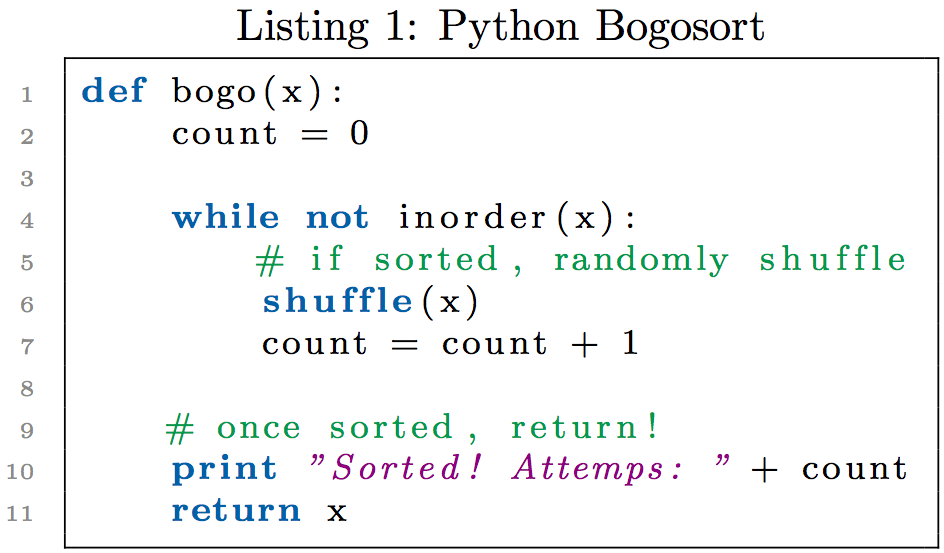
\includegraphics[width=0.85\textwidth]{Examples/9-listings.png}
	\end{center}
\end{frame}

\section{BibTex}
\begin{frame} \frametitle{Bibliographies with BibTeX}
  \begin{enumerate}
    \item Create a bibliography (.bib) file\\
    \lstinputlisting[firstline=6, lastline=14]{Examples/10-bibtex.bib} 
    \item Cite source:\\
    	\snip{cite.tex}
    \item  Include at end of document: \\
    	\snip{bibstyle.tex}
	\item Compile (with BibTeX)

  \end{enumerate}
  \note{
  	- bib entries all follow this general format: (at)type, the identifier you choose, then a comma separated key-value list.  All are optional.\\
	- note that to cite, use the same name that is specified as first argument (Meyer2000, in this case)\\
	- note the lack of the .bib extension on the bib filename\\
	- I've never used anything other than ``plain''.}
\end{frame}

\begin{frame} \frametitle{Compiling with BibTeX}
    \begin{itemize}
        \item Recommended method, according to \texttt{\href{http://www.bibtex.org/Using/}{www.bibtex.org}}\texttt{\footnotesize\\
        \ \ \ \ 1. pdflatex mydocument\\
        \ \ \ \ 2. bibtex mybib\\
        \ \ \ \ 3. pdflatex mydocument\\
        \ \ \ \ 4. pdflatex mydocument\\
        }
        \item Don't like that?\\
        \ \ \ \ \ \ \texttt{\footnotesize\url{http://users.phys.psu.edu/~collins/latexmk/}}
    \end{itemize}
    \note{ 
    - this is terrible and ugly and there is no good way around it.\\
    
    Why?\\
        1. document with question marks for unknown references\\
        2. parse all the .bib files, generate info regarding references\\
        3. generate document with references in the correct places\\
        4. just in case if adding references broke page numbering\\
    }
\end{frame}

\begin{frame} \frametitle{BibTeX Demo}
    BibTeX citations are widely used in academics and available for free from ACM digital library, IEEE Xplore, and other libraries.\\
    \begin{itemize}
        \item \texttt{\href{http://goo.gl/oyeyzr}{ACM demo}
        \item \href {http://goo.gl/4QycmW}{IEEE Xplore Demo}} 
    \end{itemize}
    Example bibliography and cited document:
    \begin{itemize}
        \item \texttt{\href{run:Examples/10-bibtex.bib}{bibliography}
        \item \href{run:Examples/10-bibtex.tex}{cited document} 
        \item \href{run:Examples/10-bibtex.pdf}{final output}}
    \end{itemize}
    \note{
    \textbf{demo} show how to get citations from ACM/Xplore\\
    \textbf{demo} show example files quickly}
\end{frame}

\section{Conclusion}

\begin{frame}\frametitle{Additional Resources}
\begin{itemize}
\item All example code listed in this presentation (anything with line numbers) located in Examples/
\item Many additional examples (omitted from presentation) located in Appendix/
	\begin{itemize}
		\item Custom sizing
		\item Algorithms
		\item Defining new functions
		\item Custom header files
	\end{itemize}
\item The source code from this presentation	
\item First places to go for help:\\
\begin{itemize}
\item \url{http://detexify.kirelabs.org/}
\item \url{http://en.wikibooks.org/wiki/LaTeX}
\item \url{http://tex.stackexchange.com/}
\item \url{http://lmgtfy.com/?q=listings+latex}
\end{itemize}
\end{itemize}
\note{
- there are working example that include all code seen in this presentation (snippets were shown)\\
- entire directory of other examples including an already-written header file that contains useful functions and packages\\
- if interested in presentations, see source code for this one.  Uses a package called Beamer designed for presentations.\\
- between wikibooks and stack exchange, 99\% of my questions are answered.}
\end{frame}

\begin{frame} \frametitle{Questions?}
\begin{center}
	
\includegraphics[width=.7\textwidth]{Resources/doge.jpg}
	\end{center}
\end{frame}

\end{document}
       
